\documentclass[final, xcolor=pdftex, dvipsnames, table, aspectratio=169, 14pt]{beamer}
\usepackage[utf8]{inputenc}
\usepackage[english]{babel}
\usepackage[T1]{fontenc}
\usepackage{droid}
\usepackage{pgf-pie}
\usepackage{hyperref}
\usepackage{multicol}
\renewcommand{\sum}{170}

\usetikzlibrary{decorations.pathreplacing,positioning, arrows.meta}
\frenchspacing % Don't put two spaces after periods.
\usepackage{pgfpages}

\setbeameroption{hide notes}

\setbeamerfont{note date}{size=\scriptsize}
\setbeamerfont{note title}{size=\footnotesize}
\setbeamerfont{note page}{size=\footnotesize}

\usepackage{graphicx}
\usetheme{DarkConsole}

\begin{document}

% The metadata of the presentation
\title[Worlds]{Worlds}
\subtitle[]{A Distributed MMO}
\author[]{Ryan Walker\footnote{\texttt{ryan.cjw@gmail.com, \href{worldsmmo.com}{worldsmmo.com}}}}
\date{\today} % Replace with date of the presentation


\begin{frame}
  \maketitle
  \note{
    I'm the note from the title page.
  }
\end{frame}

\begin{frame}{Outline} % This is the list of content with all the sections of the presentation
\small
\begin{multicols}{2}
\tableofcontents
\end{multicols}
\end{frame}

\section{Identity}
\begin{frame}{Identity}
\[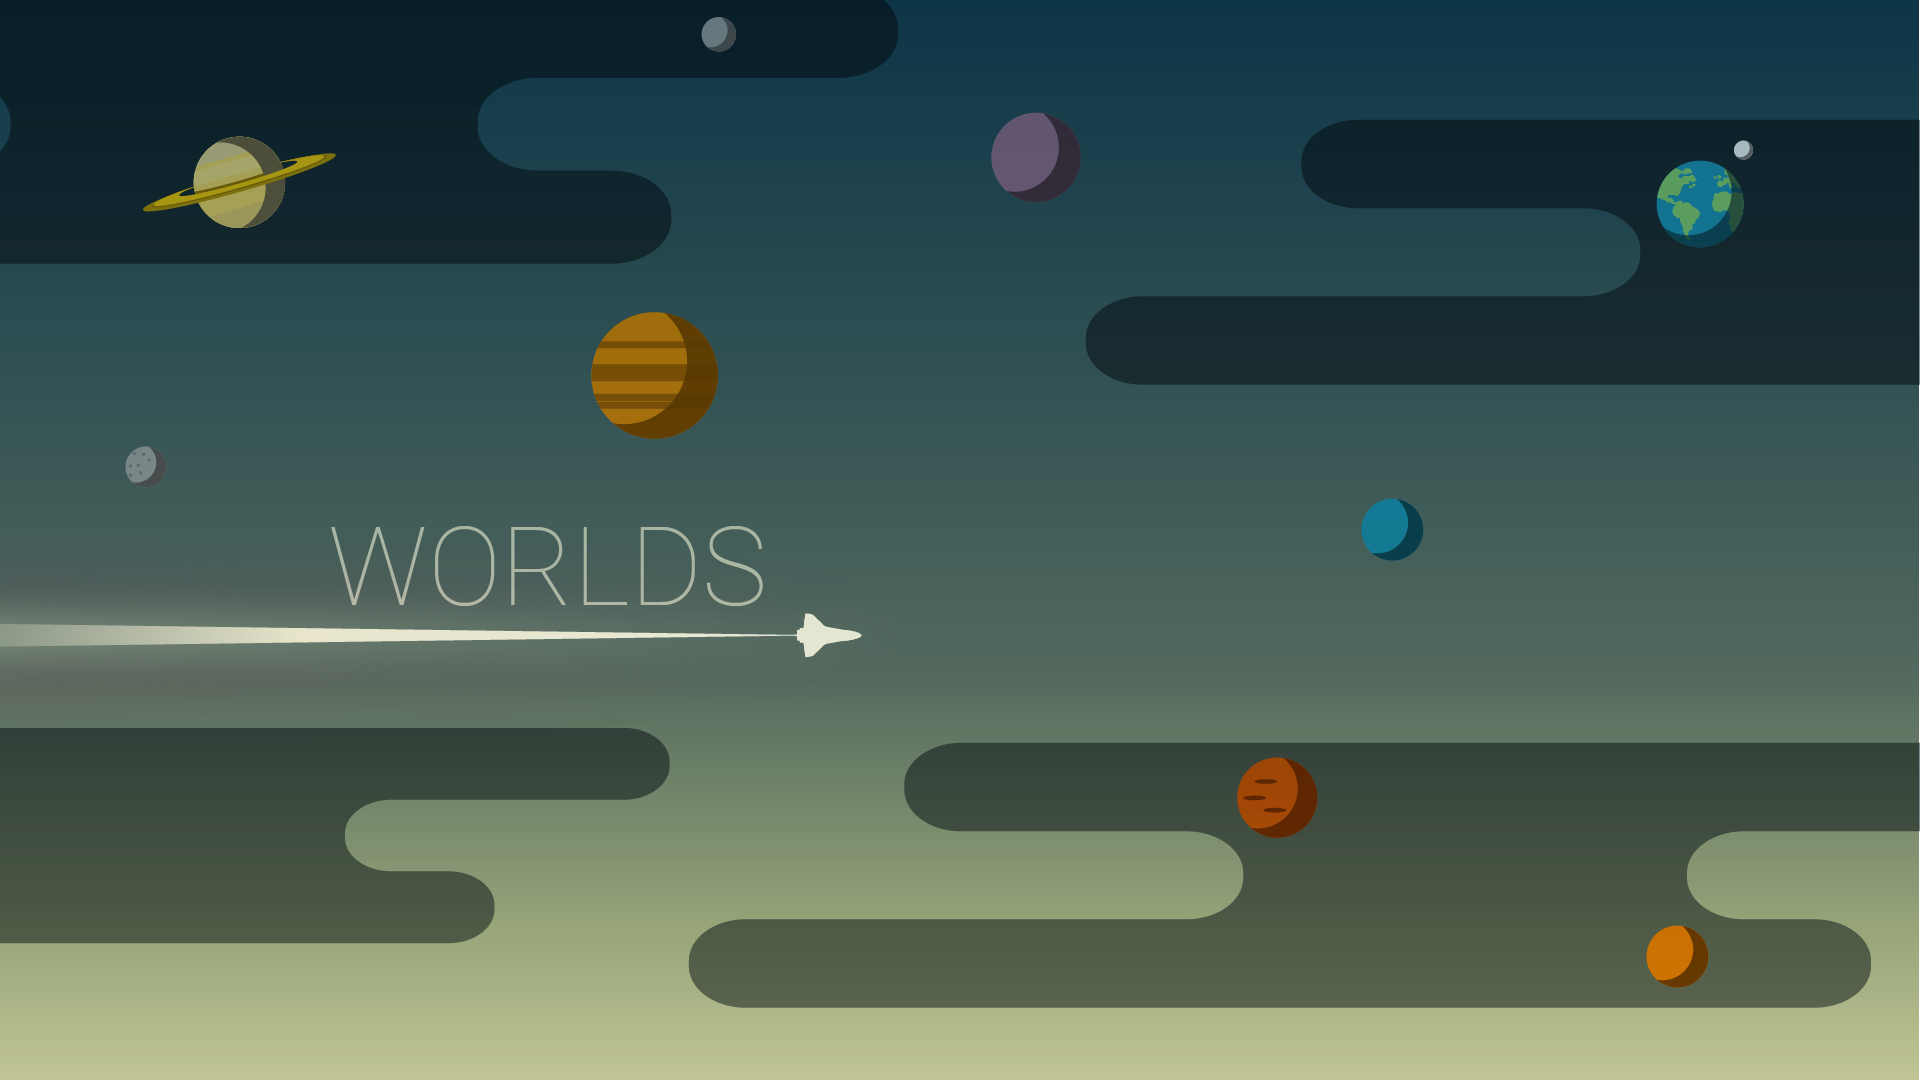
\includegraphics[scale=0.15, trim={0 4cm  0 4cm},clip]{Header.png}\] 
Worlds is the economic backbone for a distributed massively multiplayer online game (MMO). Is enables players to move digital assets throughout multiple games forming one congruent universe. 
\end{frame}

\section{Mission}
\begin{frame}{Mission}
Worlds will be the first open and scaleable infrastructure for building an unbounded MMO. This platform will lead to the organic growth of the largest online game ever created.
\end{frame}

\section{Problem}
\begin{frame}{Problem}
% The economy of an open world comes down to game theory. 
Allowing any user to modify the source code of a game enables them to create unbounded resources; this creates an economic imbalance. 
\\~\\
To combat this, Worlds implements a smart contract to manage the resources ensuring that digital wealth cannot be created from nothing.  
\end{frame}

\section{Infrastructure}
\begin{frame}{Infrastructure}
Worlds has two components: 
\begin{enumerate}
\item Worlds smart contract
\item Worlds Engine (wallet)
\end{enumerate}
\vfill 
I have forked an open source version of Minecraft to demonstrates the functionality of Worlds. See link below for a demonstration.
\\~\\
\footnotesize
Full Stack Demo:
\href{https://www.youtube.com/watch?v=OrOZVr-j92A}{youtube.com/watch?v=OrOZVr-j92A}\label{vid}
%\\
%Github:
%\href{https://github.com/Machine-Hum/Worlds}{github.com/Machine-Hum/Worlds}

\end{frame}

\begin{frame}{Infrastructure}
Explain how anyone can build their own world and plug it into the universe.
\end{frame}

\section{Startup}
\begin{frame}{Startup}
Smaller communities will initially be targeted. Simple open source games are a good starting point. The initial vision is several smaller integrated Worlds to prove the concept and build a community.
\\~\\
Worlds does not suffer from the chicken and egg problem. Even a small number of "Worlds" would create an interesting experience. Once a userbase is established, the universe will scale organically.
\end{frame}


%\section{Target}
%\begin{frame}{Target}
%To get the ball rolling, smaller communities will be targeted. Simple open source games such as Minecraft (which is currently implemented) are a good starting point. The initial vision is several smaller integrated Worlds to prove the concept and build a community.
%\end{frame}
%
%\section{Market}
%\begin{frame}{Market}
%Unlike several cyrpto projects, Worlds does not suffer from the chicken and egg problem. A small implementation of ten or so Worlds maintained by independent parties would create an interesting experience. The universe will organically scale from that, funding (and later tokens) will be given to key developers at predetermined milestones.
%\end{frame}

\section{Advantage}
\begin{frame}{Advantage}
My focus is full stack: by leveraging open source tech, I will be able to build the game clients required to fuel the initial fire. Other similar projects rely on game developers to take a leap of faith and pour valuable development time into using their platform. By contrast, to develop in Worlds, coding skills aren't required. 
\end{frame}

\begin{frame}{Advantage}
Worlds is 100\% open source and transparent. I want to build tools to enable my vision, and then use those tools to show people what is possible.
\end{frame}

\begin{frame}{Advantage}
Worlds is built on EOS, which has the rapid finality required for a game. 
\end{frame}

%\begin{frame}{Disadvantages}
%I hate this slide. Marketing is a necessary evil. I believe that strong marketing without strong tech is a fundraising mechanism. While strong marketing with strong tech is a community building mechanism. I have been focusing on the technology up until now, however in the future once I build out the tools there will be a requirement for marketing. Without funding, success will be difficult.  
%\end{frame}

\section{Roadmap}

\begin{frame}{Roadmap}


\begin{center}
\begin{tikzpicture}
\draw[thick, -latex] (-0.5,0) -- (10.5,0);
%big ticks
\foreach \x in {0,4,8}
\draw (\x cm,5pt) -- (\x cm,-5pt);
%little ticks
\foreach \x in {1,2,3,5,6,7,9,10}
\draw (\x cm,3pt) -- (\x cm,-3pt);
%yr labels
\foreach \x/\descr in {0/2018,4/2019,8/2020}
\node[font=\scriptsize, text height=1.75ex,
text depth=.5ex] at (\x,0.4) {$\descr$};
%events

\draw[chartreuse, line width=4pt] (1,0) -- +(0.5,0)node[below left=2pt and 10pt,rotate=45]{\scriptsize Project Conceptualized};

\draw[chartreuse, line width=4pt] (2.25,0) -- +(0.2,0)node[below left=2pt and 10pt,rotate=45]{\scriptsize EOS Selected / Mainnet launch};

\draw[chartreuse, line width=4pt] (3,0) -- +(0.2,0)node[below left=2pt and 10pt,rotate=45]{\scriptsize Paper Complete};

\draw[chartreuse, line width=4pt] (3.75,0) -- +(0.2,0)node[below left=2pt and 10pt,rotate=45]{\scriptsize First Item Created};

\draw[chartreuse, line width=4pt] (4.2,0) -- +(0.2,0)node[below left=2pt and 10pt,rotate=45]{\scriptsize Minetest Forked};

\draw[chartreuse, line width=4pt] (5.75,0) -- +(0.2,0)node[below left=2pt and 10pt,rotate=45]{\scriptsize Wallet/Engine Functional};

\draw[chartreuse, line width=4pt] (6.5,0) -- +(0.2,0)node[below left=2pt and 10pt,rotate=45]{\scriptsize Full Stack Demo};

\draw[chartreuse, line width=4pt] (8,0) -- +(0.2,0)node[below left=2pt and 10pt,rotate=45]{\scriptsize Full Testnet Deployment};

\draw[chartreuse, line width=4pt] (9,0) -- +(0.2,0)node[below left=2pt and 10pt,rotate=45]{\scriptsize First World Deployed};

\draw[chartreuse, line width=4pt] (10,0) -- +(0.2,0)node[below left=2pt and 10pt,rotate=45]{\scriptsize Mainnet Deployment};

\end{tikzpicture}
\end{center}
\end{frame}

\section{Buisness / Token Model}
\begin{frame}{Token Cap Table}


\begin{figure}[H]
\begin{center}
\begin{tikzpicture}
\footnotesize
\pie [rotate = 180, radius=1.5, color={indigo}, explode=0.2]
{10/Kept for the team,
 40/Given to developers, 
 10/Sold to Private Investment,
 40/Community Airdrop
}
\end{tikzpicture}
\end{center}
\end{figure}
The token cap model is geared towards stimulating initial project growth within the community.
\end{frame}

\section{Fundraising}
\begin{frame}{Fundraising}

\begin{figure}[H]
Fundraising target for year one: \textbf{\$\sum k}
\begin{center}
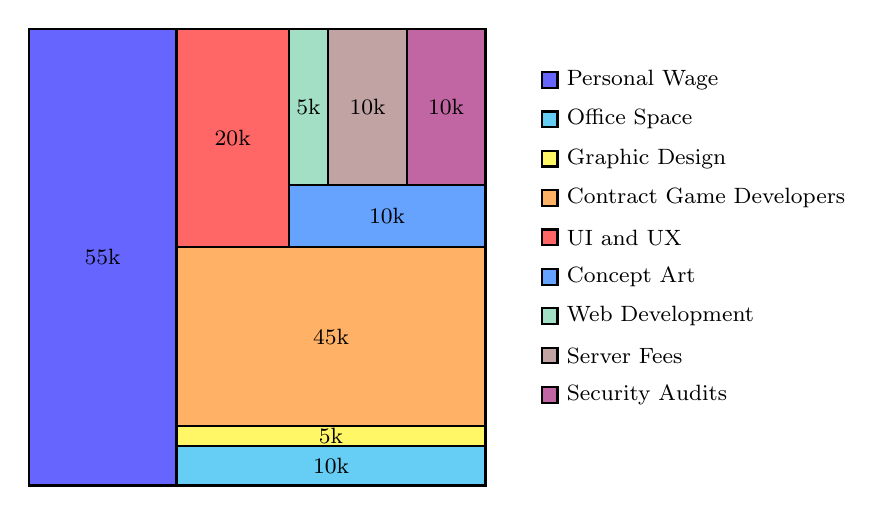
\begin{tikzpicture}
\footnotesize
\pie [square, radius=2.9, text=legend, after number = {k}, sum=\sum]
{55/Personal Wage,
 10/Office Space, 
 5/Graphic Design,
 45/Contract Game Developers,
 20/UI and UX ,
 10/Concept Art,
 5/Web Development,
 10/Server Fees,
 10/Security Audits
}
\end{tikzpicture}
\label{funding}
\end{center}
\end{figure}

\end{frame}
\begin{frame}{Fundraising}
The existing development has been done on my free time. I am looking to raise seed funding to make this my full time job. I am offering 5\% of the total supply WOR for \$\sum k. Following the mainnet launch, I will be raising a series A.
\end{frame}

\begin{frame}{Thank You}
I appreciate your consideration. Please reach out with any questions or feedback!
\\ \vfill
\begin{minipage}{0.5\textwidth}
\[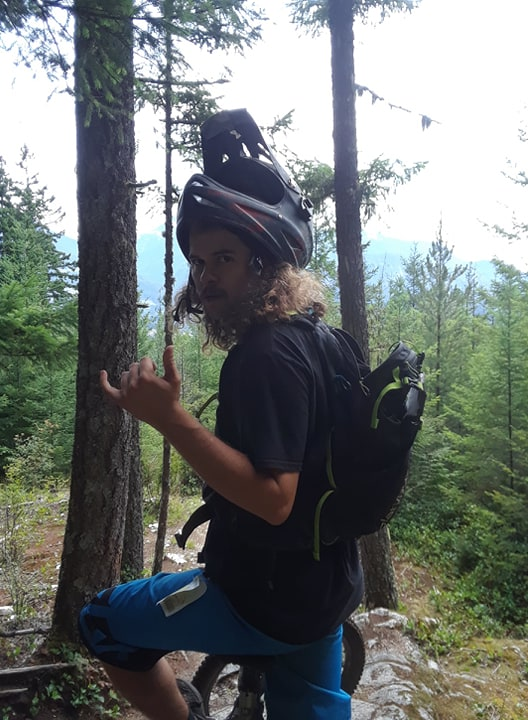
\includegraphics[scale=0.25, trim={0 2cm  0 2cm},clip]{me.jpg}\] 
\end{minipage}%
\begin{minipage}{0.5\textwidth}
Ryan Walker \\ Ryan.cjw@gmail.com \\  
\\~\\
\href{worldsmmo.com}{worldsmmo.com} \\ \href{https://www.youtube.com/watch?v=OrOZVr-j92A}{Demo}
\end{minipage}
\end{frame}

\end{document}
